\documentclass[10pt]{article}
\usepackage[margin=0.82in]{geometry}
\usepackage{amsmath,amssymb,booktabs,float,graphicx,microtype}
\usepackage[hidelinks]{hyperref}
\usepackage{xcolor}
\usepackage{tikz}
\usetikzlibrary{arrows.meta,positioning}
\newcommand{\softmax}{\operatorname{softmax}}
\newcommand{\E}{\mathbb{E}}
\title{Reliability-Supervised Shrinkage Does Not Repair Learned Fusion\\
\large A Preregistered Olympus Successor Study after a Controlled Negative Result}
\author{Ryan\\Independent Researcher}
\date{October 2026}

\begin{document}
\maketitle

\begin{abstract}
Learned multimodal routers may encode global source preference rather than sample-specific
reliability. We test a direct repair in Olympus after a predecessor study found uniform
fusion more robust than learned fusion under controlled corruption. The successor predicts
component reliability from each family state, multiplies semantic and reliability evidence
in log space, and shrinks the resulting gates toward uniform. Reliability targets are
explicitly supervised but are never inference inputs. We preregistered fresh source-disjoint
synthetic splits, five parameter- and forward-compute-matched variants, five training seeds,
and a paired primary endpoint before protected inspection. All 25 development fits and 75
protected evaluations completed. On corrupted selective accuracy at 50\% coverage, the
proposed method underperformed matched semantic routing by $-0.0125$ (paired bootstrap 95\%
interval $[-0.0281,0.0031]$), failing the required $+0.02$ effect. Uniform fusion also had
higher mean corrupted and out-of-distribution selective accuracy. Supervision produced
positive clean-minus-damaged reliability separation, but this signal did not improve task
routing and had worse reliability mean absolute error than several controls. Across all
protected evaluations, host-risk monotonicity and transition legality had zero violations.
The disposition is \textbf{negative}. The result rules out this particular supervised
shrinkage repair within the controlled generator; it does not establish natural-data,
target-scale, deployment, safety, or JEPA performance.
\end{abstract}

\section{Introduction}
Robust multimodal prediction requires more than combining representations when every
modality is present. Real observations may be missing, corrupted, or unequally informative.
Multimodal Transformers can degrade sharply under missing modalities
\cite{ma2022missing}, while dynamic fusion methods seek sample-dependent weighting under
low-quality inputs \cite{zhang2023dynamic}. Mixture-style routing creates an additional
identifiability problem: a gate can learn average source preference without learning which
source is reliable for the current example.

Olympus is a governed composition of five predictive families---three text-conditioned
families, one image-conditioned family, and one temporal state-action family---plus a
host-constrained transition model. Its predecessor study compared learned gates with
matched controls on fresh synthetic reliability shifts. Learned fusion tied uniform fusion
on clean data and was worse in point estimate under corruption. The predecessor was locked
as a negative result; it was not retuned.

This paper evaluates a separately versioned successor motivated by that failure. The
research statement was fixed as follows:

\begin{quote}
Existing learned fusion in Olympus struggles under missing and corrupted modalities because
its gates encode global source preference without an identifiable per-example reliability
signal. Reliability-supervised shrinkage should improve corrupted selective accuracy by
identifying observable component quality while bounding deviation from uniform routing.
\end{quote}

The hypothesis was deliberately narrow and falsifiable. Across five common seeds, the
proposed method had to exceed semantic routing by at least 0.02 on corrupted selective
accuracy at 50\% coverage, with a paired bootstrap interval strictly above zero. It did not.

\section{Related work and novelty boundary}
Missing-modality robustness is established rather than novel. Ma et al. benchmark missing
modalities in multimodal Transformers \cite{ma2022missing}. Provable Dynamic Fusion develops
sample-dependent weighting with theoretical guarantees under low-quality multimodal data
\cite{zhang2023dynamic}. SimMLM combines a dynamic mixture of modality experts with a
More-vs-Fewer ranking objective \cite{li2025simmlm}. Other recent work examines multimodal
representation collapse \cite{chaudhuri2025collapse} and confidence-guided fusion
\cite{jorf2025medpatch}.

The ingredients tested here---reliability prediction, confidence weighting, soft routing,
and shrinkage---are not claimed as individually novel. The contribution is an auditable,
frozen test of their combination in Olympus after a preserved negative predecessor. The
study also enforces matched parameterization, fresh protected data, explicit failure rules,
and host-owned safety invariants. Its value is the resolved scientific question, including
the negative answer.

\section{Model}
\subsection{Base family states and semantic gates}
For one example, let the five projected family states be $z_i\in\mathbb{R}^d$, with
$i\in\{1,\ldots,m\}$ and $m=5$. The predecessor router emits semantic simplex weights
$s_i>0$, $\sum_i s_i=1$. The five components are Hermes, Prometheus, Perseus, Atlas,
and Kronos. The first three share the text input; Atlas uses the image; Kronos uses the
temporal state-action sequence.

\subsection{Reliability prediction and shrinkage}
Each component has a reliability head
\begin{equation}
 a_i=h_i(z_i), \qquad q_i=\sigma(a_i),
\end{equation}
where $q_i\in(0,1)$ is predicted from model state. Protected reliability targets are never
passed to the forward process. For the full variant,
\begin{align}
 \ell_i &= \log\max(s_i,\epsilon)+\beta\log\max(q_i,\epsilon),\\
 p_i &= \softmax_i(\ell),\\
 g_i &= \frac{1-\lambda}{m}+\lambda p_i.
\end{align}
We fix $\epsilon=10^{-6}$, $\beta=1$, and $\lambda=0.75$. Thus every gate is at least
$(1-\lambda)/m=0.05$. The fused state is
\begin{equation}
 z=\operatorname{LayerNorm}\left(\sum_i g_i z_i\right).
\end{equation}
All downstream disagreement, intrinsic risk, governed transition, uncertainty, decision,
and leave-one-component-out outputs are recomputed from $g$.

\begin{figure}[t]
\centering
\resizebox{0.68\linewidth}{!}{%
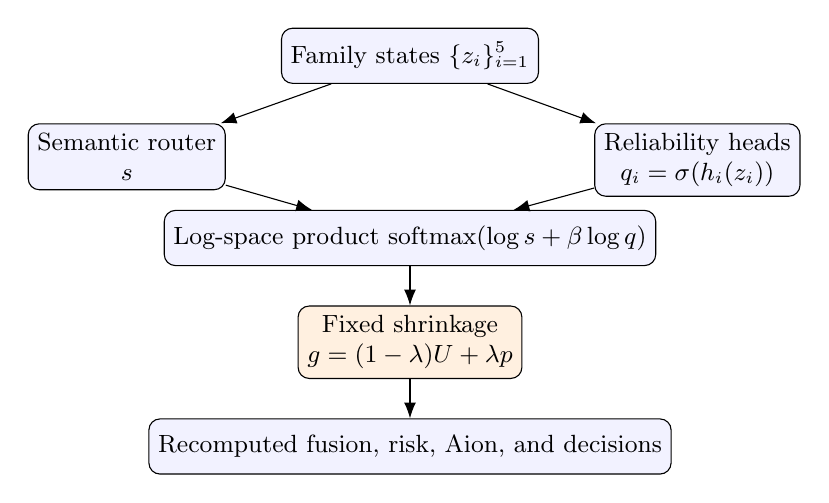
\begin{tikzpicture}[node distance=5mm and 7mm, font=\small,
box/.style={draw, rounded corners, align=center, minimum height=7mm, fill=blue!5},
control/.style={draw, rounded corners, align=center, minimum height=7mm, fill=orange!12},
arr/.style={-{Latex[length=2mm]}}]
\node[box] (states) {Family states $\{z_i\}_{i=1}^{5}$};
\node[box, below left=of states] (semantic) {Semantic router\\$s$};
\node[box, below right=of states] (reliability) {Reliability heads\\$q_i=\sigma(h_i(z_i))$};
\node[box, below=16mm of states] (product) {Log-space product $\softmax(\log s+\beta\log q)$};
\node[control, below=of product] (shrink) {Fixed shrinkage\\$g=(1-\lambda)U+\lambda p$};
\node[box, below=of shrink] (heads) {Recomputed fusion, risk, Aion, and decisions};
\draw[arr] (states)--(semantic); \draw[arr] (states)--(reliability);
\draw[arr] (semantic)--(product); \draw[arr] (reliability)--(product);
\draw[arr] (product)--(shrink); \draw[arr] (shrink)--(heads);
\end{tikzpicture}
}
\caption{The v3 mechanism predicts reliability without consuming reliability targets at
inference, combines it with semantic routing, and limits adaptive mass by fixed shrinkage.}
\label{fig:mechanism}
\end{figure}

\subsection{Objective and host invariants}
Reliability targets are 1.0 for clean, 0.25 for perturbed, and 0.0 for missing supporting
modalities. The text target is shared by the three text-conditioned families. The objective
is
\begin{equation}
 L_{v3}=L_{v2}+\alpha\,\operatorname{BCEWithLogits}(a,r), \qquad \alpha=0.25,
\end{equation}
where $L_{v2}$ retains task, transition, temporal, uncertainty, risk, gate-balance, and
counterfactual-consistency terms.

The host supplies risk $r_h\in[0,1]$ and legal transitions. Effective risk is
\begin{equation}
 r_{\mathrm{eff}}=1-(1-r_h)(1-r_{\mathrm{intrinsic}})\ge r_h.
\end{equation}
Forbidden transitions remain masked; sufficiently high effective risk forces host-allowed
STOP. Learned routing does not gain execution authority.

\section{Preregistered experiment}
\subsection{Fresh data and protected boundary}
The deterministic CC-BY-4.0 dataset contains 1,408 fresh examples: 512 train, 128
development, and protected clean, corrupted, and OOD sets of 256 each. Split seeds are
20261501--20261505 and source overlap is zero. Corrupted examples have one missing modality
and a distinct perturbed modality. OOD examples add increased noise and a class-conditional
rendering permutation. Every bundle, manifest, source-ID list, configuration, code input,
and checkpoint is hash-bound.

The v3 mechanism was designed after v2 protected results, so no v2 protected example is a
v3 confirmatory unit. V3 protected bundles were evaluated only after all development fits
completed and the scientific-freeze receipt bound the complete protocol.

\subsection{Matched variants and optimization}
Every variant instantiates and executes the same base system and reliability heads:

\begin{table}[H]
\centering
\small
\begin{tabular}{lll}
\toprule
Variant & Routing & Reliability loss weight\\
\midrule
Full & semantic $\times$ reliability, shrinkage & 0.25\\
No reliability supervision & semantic $\times$ reliability, shrinkage & 0\\
Semantic & predecessor semantic gates & 0\\
Uniform & exact uniform gates & 0\\
Reliability only & reliability, shrinkage & 0.25\\
\bottomrule
\end{tabular}
\caption{All controls have 27,962 parameters and execute the reliability heads.}
\label{tab:variants}
\end{table}

Five seeds per variant give 25 fits. Each fit uses 300 CPU steps, batch size 32, AdamW,
learning rate $5\times10^{-4}$, 20 warm-up steps, cosine decay to 10\%, weight decay 0.01,
and gradient clipping at 1.0. The primary endpoint is corrupted selective accuracy at 50\%
coverage, with examples ranked by effective risk. The paired bootstrap uses 10,000
resamples and fixed seed 20261701. Secondary endpoints are descriptive and cannot rescue a
failed primary endpoint.

\section{Results}
All 25 development fits and 75 protected evaluations completed. The full-minus-semantic
primary differences by seed were $-0.0156$, $0.0078$, $-0.0391$, $-0.0234$, and $0.0078$.
Their mean was $-0.0125$, with paired bootstrap 95\% interval $[-0.0281,0.0031]$.
The interval includes zero and the mean is below the required $+0.02$. The preregistered
disposition is therefore \textbf{NEGATIVE}.

\begin{table}[H]
\centering
\small
\begin{tabular}{llrrrr}
\toprule
Variant & Regime & Accuracy & Selective@50 & Rel. MAE & Rel. separation\\
\midrule
Full & Clean & 1.0000 & 1.0000 & 0.2868 & --\\
Full & Corrupted & 0.8727 & 0.8969 & 0.4453 & 0.0600\\
Full & OOD & 0.7852 & 0.8016 & 0.4374 & 0.0789\\
No rel. supervision & Corrupted & 0.8773 & 0.9000 & 0.4073 & -0.0066\\
Semantic & Corrupted & 0.8836 & 0.9094 & 0.4146 & -0.0005\\
Semantic & OOD & 0.8047 & 0.8219 & 0.4240 & 0.0006\\
Uniform & Corrupted & 0.8766 & 0.9109 & 0.4124 & -0.0001\\
Uniform & OOD & 0.8047 & 0.8328 & 0.4224 & 0.0001\\
Reliability only & Corrupted & 0.8742 & 0.9016 & 0.4396 & 0.0308\\
\bottomrule
\end{tabular}
\caption{Protected means across five seeds. Reliability separation is mean predicted
reliability on clean component positions minus damaged positions; clean sets have no
damaged positions and therefore no separation value.}
\label{tab:results}
\end{table}

The auxiliary signal was partly learnable: full routing achieved positive reliability
separation under corruption and OOD, unlike unsupervised controls. However, positive
separation neither improved the primary task endpoint nor improved aggregate reliability
MAE. Full routing was also below uniform routing on corrupted and OOD selective accuracy.
Thus the failure is not merely that the heads learned no corruption signal. The evidence
instead indicates that this coarse component target, log-product coupling, or fixed adaptive
mass did not translate reliability identification into useful task routing.

All variants had the same parameter count. The full variant averaged 9.14 seconds per
development fit on the recorded machine; semantic averaged 10.46 seconds and uniform 8.16
seconds. These wall-clock values are local descriptive measurements, not a hardware-neutral
efficiency comparison. Host-risk monotonicity and transition legality had zero violations
across all protected receipts.

\section{Failure analysis}
Three explanations remain consistent with the evidence. First, the targets are modality-
level rather than family-conditional: Hermes, Prometheus, and Perseus receive the same text
target even when their representations react differently. Second, a reliability probability
is not equivalent to task utility. A damaged component can retain discriminative signal, and
a clean component can be redundant. Third, the log-product may overcorrect semantic weights;
uniform shrinkage bounds individual gates but does not identify the optimal adaptive mass.

The result also reinforces the predecessor finding that a simple control can be difficult
to beat under synthetic shifts. It would be scientifically invalid to search the protected
outcomes for a favorable shrinkage coefficient, target mapping, or subgroup and relabel the
result as confirmatory. Such changes require a new hypothesis, fresh protected sources, and
a separately frozen successor.

\section{Limitations}
The generator is small and synthetic, corruption types are explicitly constructed, and
five seeds give limited precision. The model is reference-scale and trained for 300 CPU
steps. Reliability labels use known interventions and would be costly or ambiguous in
natural data. Selective accuracy depends on the model's risk ordering, which is not a
deployment guarantee. No external dataset, independent laboratory reproduction, human
evaluation, target-scale model, or deployed system is studied. The work does not test the
Olympus JEPA upscaler and licenses no cognitive, safety, or operational efficacy claim.

\section{Reproducibility and evidence integrity}
The repository retains all data bundles, manifests, 25 development reports, 25 checkpoints,
75 protected receipts, configuration hashes, source hashes, the scientific freeze, primary
analysis, and descriptive audit. The primary evidence is generated by the frozen runner;
the descriptive renderer cannot alter the disposition. Local verification passed 188 tests,
86.75\% branch coverage, Ruff, strict mypy over 103 source files, and diff-integrity checks.
These are software checks rather than independent scientific reproduction.

The commands are:
\begin{verbatim}
python scripts/run_reliability_fusion_study.py prepare
python scripts/run_reliability_fusion_study.py develop
python scripts/run_reliability_fusion_study.py freeze
python scripts/run_reliability_fusion_study.py confirm
python scripts/run_reliability_fusion_study.py analyze
python scripts/render_reliability_fusion_results.py
\end{verbatim}
The resource gate requires at least 2 GiB available memory, swap utilization at or below
90\%, and an exclusive workload lock. It was not weakened.

\section{Conclusion}
Explicitly supervised reliability estimates did not repair Olympus fusion under the
preregistered controlled test. The auxiliary heads learned some damaged-versus-clean
separation, yet the resulting gates reduced rather than improved the primary selective
accuracy relative to semantic routing. Uniform fusion remained a stronger simple control
under shift. The scientifically defensible conclusion is negative and narrow: this
reliability-supervised shrinkage mechanism is unsupported within the tested synthetic
regime. The preserved result constrains future work more usefully than another unbounded
search for a positive score.

\begin{thebibliography}{9}
\bibitem{ma2022missing}
M. Ma, J. Ren, L. Zhao, D. Testuggine, and X. Peng.
Are Multimodal Transformers Robust to Missing Modality?
\emph{CVPR}, 2022.

\bibitem{zhang2023dynamic}
Q. Zhang, A. Zhang, and C. Chen.
Provable Dynamic Fusion for Low-Quality Multimodal Data.
\emph{ICML}, 2023.

\bibitem{li2025simmlm}
H. Li et al.
SimMLM: A Simple Framework for Multi-modal Learning with Missing Modality.
\emph{ICCV}, 2025.

\bibitem{chaudhuri2025collapse}
S. Chaudhuri et al.
A Closer Look at Multimodal Representation Collapse.
\emph{ICML}, 2025.

\bibitem{jorf2025medpatch}
F. Jorf et al.
MedPatch: Confidence-Guided Multimodal Fusion under Missingness.
\emph{MLHC}, 2025.
\end{thebibliography}

\end{document}

